\lstinputlisting[language=bash,basicstyle=\small]{python_codes/fieldstone_45/keywords}

\begin{center}
Code at \url{https://github.com/cedrict/fieldstone/tree/master/python_codes/fieldstone_45}
\end{center}

\par\noindent\rule{\textwidth}{0.4pt}
%%%%%%%%%%%%%%%%%%%%%%%%%%%%%%%%%%%%%%%%%%%%%%%%%%%%%%%%%%%%%%%%%%%%%%%%%%%%%%%%%%%%%%%%%%%%

This experiment is based on the benchmark paper by van Keken et al, 2008 \cite{vack08}.
It shares similarities with the 
time dehydration processes in subduction zones work by Magni et al., 2014 \cite{mabv14} and 
the 3D corner flow study of Plunder et al, 2018\cite{pltv18}. See also Cerpa et al, 2017 \cite{ceww17}
for a study of fluid migration in the mantle wedge.

The domain is $660\text{km}\times 600\text{km}$. Note that in the original paper the 
origin of the coordinate system is at the top left while it is at the lower left corner 
in our code.

\begin{center}
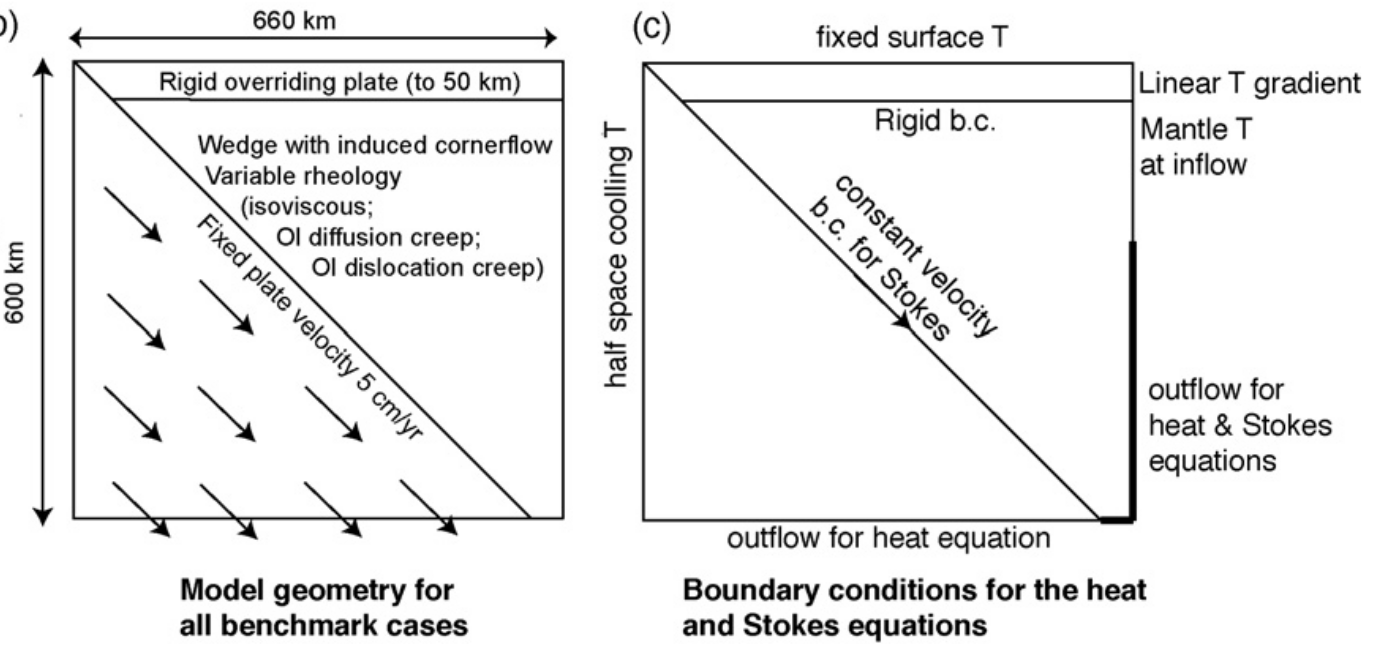
\includegraphics[width=14cm]{python_codes/fieldstone_45/images/setup1}
\end{center}

As shown in the figure above, 
the inflow boundaries (at both wedge and trench sides) and top of the model 
have prescribed temperature. The wedge is assumed to be an incompressible fluid that
is driven only by the kinematic forcing of the slab. The wedge is
confined by the top of the slab and the base of the rigid overriding
plate (located at a depth of $50\text{km}$). 
The boundary conditions for the wedge are no-slip below the overriding plate and constant velocity
along the top of the slab. The velocity boundary conditions for the
boundaries of the wedge are either provided by the Batchelor cornerflow 
solution (cases 1a and 1b) or based on free inflow/outflow
boundaries. The velocity field is discontinuous between the slab
and the overriding plate.
The velocity in the slab is constant (5cm/yr) and it dips at a $45\degree$ angle
There is no radiogenic of shear heating.


The flow is assumed to be incompressible and buoyancy effects are neglected.
All the experiments shown in the paper are at steady state , i.e. the 
temperature field satisfies:
\begin{equation}
\rho C_p \vec\upnu\cdot\vec\nabla T = \vec\nabla\cdot (k\vec\nabla T)
\end{equation}
In the paper a simplified diffusion creep formulation is adopted and the 
effective diffusion creep viscosity is computed as follows:
\[
\eta_{\text{diff}}=A_{\text{diff}} \exp \frac{Q_{\text{diff}}}{RT}
\]
The dislocation creep effective viscosity is given by
\[
\eta_{\text{disl}}=
A_{\text{disl}} \dot\varepsilon^{(1-n)/n} \exp \frac{Q_{\text{disl}}}{nRT}
\]
Note that in both the activation volume has been set to zero, which decouples pressure
from the effective viscosities.
Both effective viscosities are limited with a maximum viscosity 
as follows:
\[
\eta_{\text{diff}}^\star = \left( \frac{1}{\eta_{\text{diff}}} +\frac{1}{\eta_{max}}  \right)
\qquad
\eta_{\text{disl}}^\star = \left( \frac{1}{\eta_{\text{disl}}} +\frac{1}{\eta_{max}}  \right)
\]

The top boundary condition is $T_{top} = T(y = L_y) = 273 K$. 
At the inflow boundary of the wedge (i.e. where $u<0$)\footnote{Think
about it: it makes little sense to prescribe a temperature where the fluid is leaving the domain} 
temperature is fixed at $T_0 = 1573 K$ 
and a linear geotherm is used at the left hand boundary of the overriding
plate from 0 to 50 km depth. The temperature at the slab inflow
boundary is described by an error-function solution for half-space
cooling for 50 Myr:
\[
T(x=0,y)=T_{top}+(T_0-T_{top}) \text{erf} \frac{L_y-y}{2\sqrt{\kappa t_{50}}}
\]
where $t_{50}$ is the age of the slab. 

At the slab and wedge outflow boundaries we prescribe
the natural boundary condition (zero curvature) for the heat equation.

the original paper considers multiple cases:
\begin{itemize}
\item Case 1a: analytical cornerflow model. The wedge flow is prescribed by
the analytical expression for cornerflow \cite{batchelor}, so that we do not need to 
solve for the Stokes equations, only the energy equation.
\item Case 1b: dynamical flow in isoviscous wedge I
This case is the same as 1a, except that the solution for the wedge
flow is determined by solving the Stokes equations 
while the Batchelor solution is imposed on the inflow and outflow boundaries.
This case tests the ability of the numerical method to accurately 
reproduce the corner flow solution.

\item Case 1c: dynamical flow in isoviscous wedge II. Same as case 1b, but with stress-free 
boundary conditions on the mantle wedge.

\item Case 2a: dynamical flow with diffusion creep
\item Case 2b: dynamical flow with dislocation creep

\end{itemize}

The temperature field as discreted values $T_{ij}$ on
an equidistant grid with $6\text{km}$ spacing, which is a $111\times101$ 
matrix stored row-wise starting in the top left corner. 
From this grid the following measurements are extracted for direct comparison:

\begin{enumerate}
\item the temperature $T_{11,11}$ which is at coordinates $(60, 60\text{km})$ 
and just down-stream from the corner point. This provides therefore
one of the most critical tests of accuracy of the numerical codes;

\item the L2 norm of the slab-wedge interface temperature between
0 and 210 km depth defined by
\[
T_{\text{slab}} = \sqrt{\frac{1}{36}\sum_{i=1}^{36} T_{ii}^2}
\]

\item the L2 norm of the temperature in the triangular part of the
tip of the wedge, between 54 and 120 km depth:
\[
T_{\text{wedge}} = \sqrt{ \frac{1}{78} \sum_{i=10}^{21} \sum_{j=10}^i T_{ij}^2}
\]

\end{enumerate}

\newpage
%----------------------------------
\subsubsection*{Results for case 1a}

\begin{center}
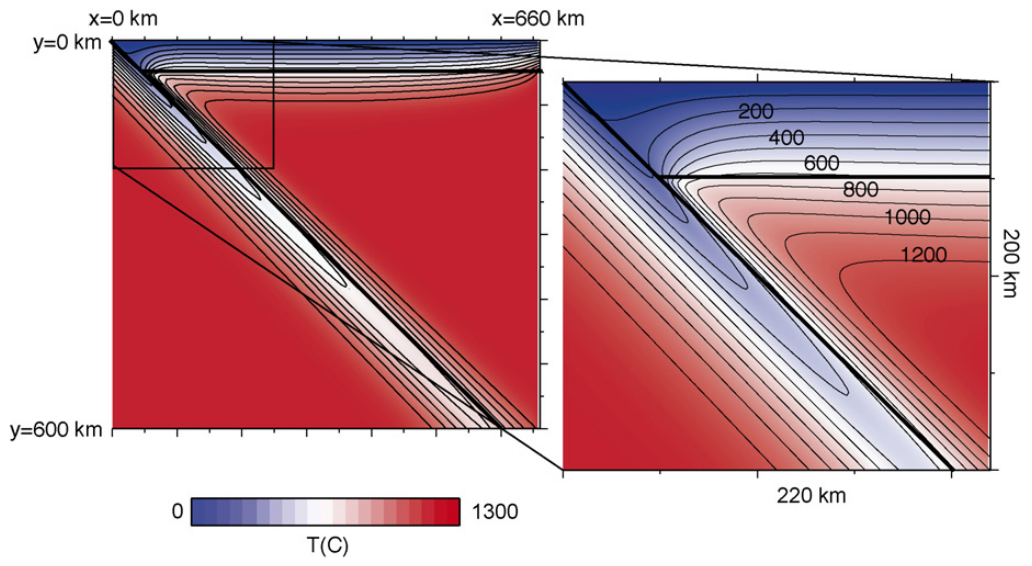
\includegraphics[width=8cm]{python_codes/fieldstone_45/images/vack08_0}
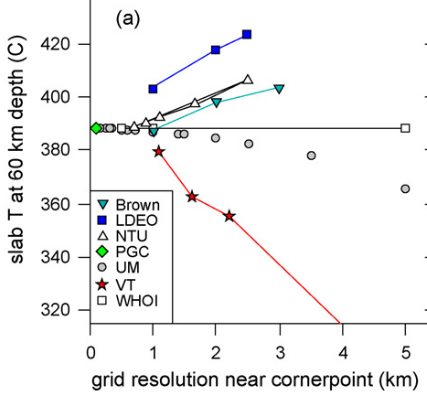
\includegraphics[width=5cm]{python_codes/fieldstone_45/images/vack08_1}\\
{\small (a) Temperature prediction for case 1a. The bold lines indicate the top of the slab and base of the overriding plate. (b) Close up of the top left part of
the model. Figures taken from \cite{vack08}.}
\end{center}


\begin{center}
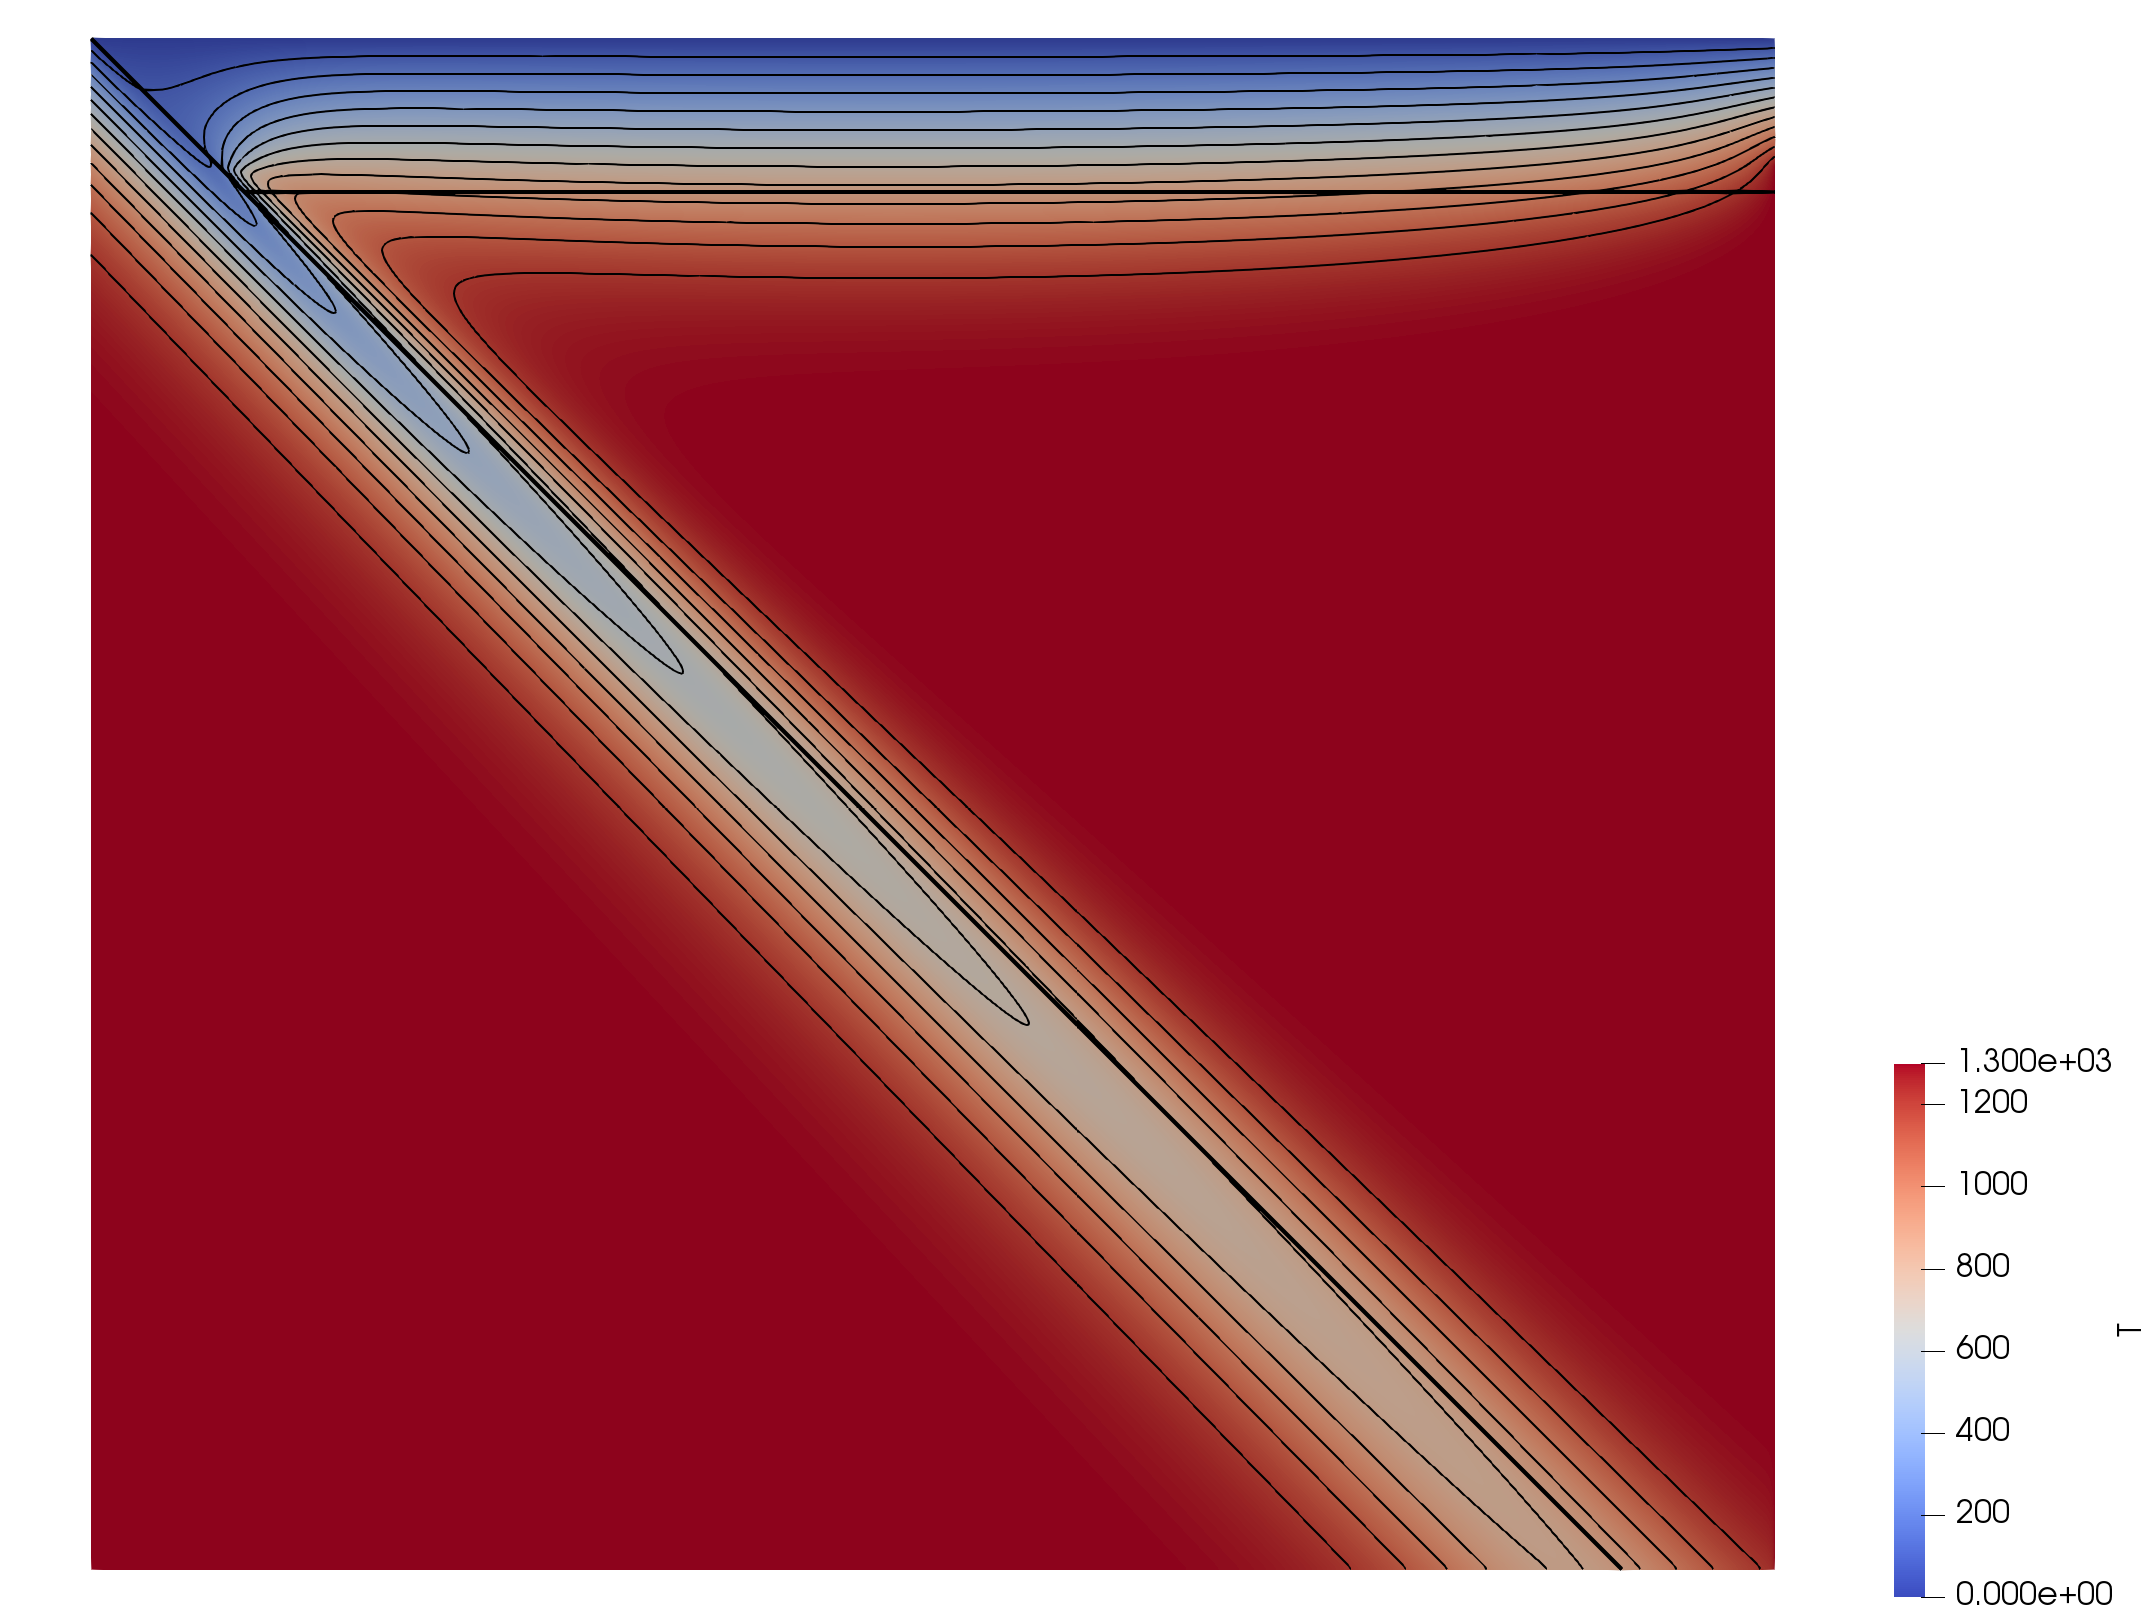
\includegraphics[width=7cm]{python_codes/fieldstone_45/images/temp}
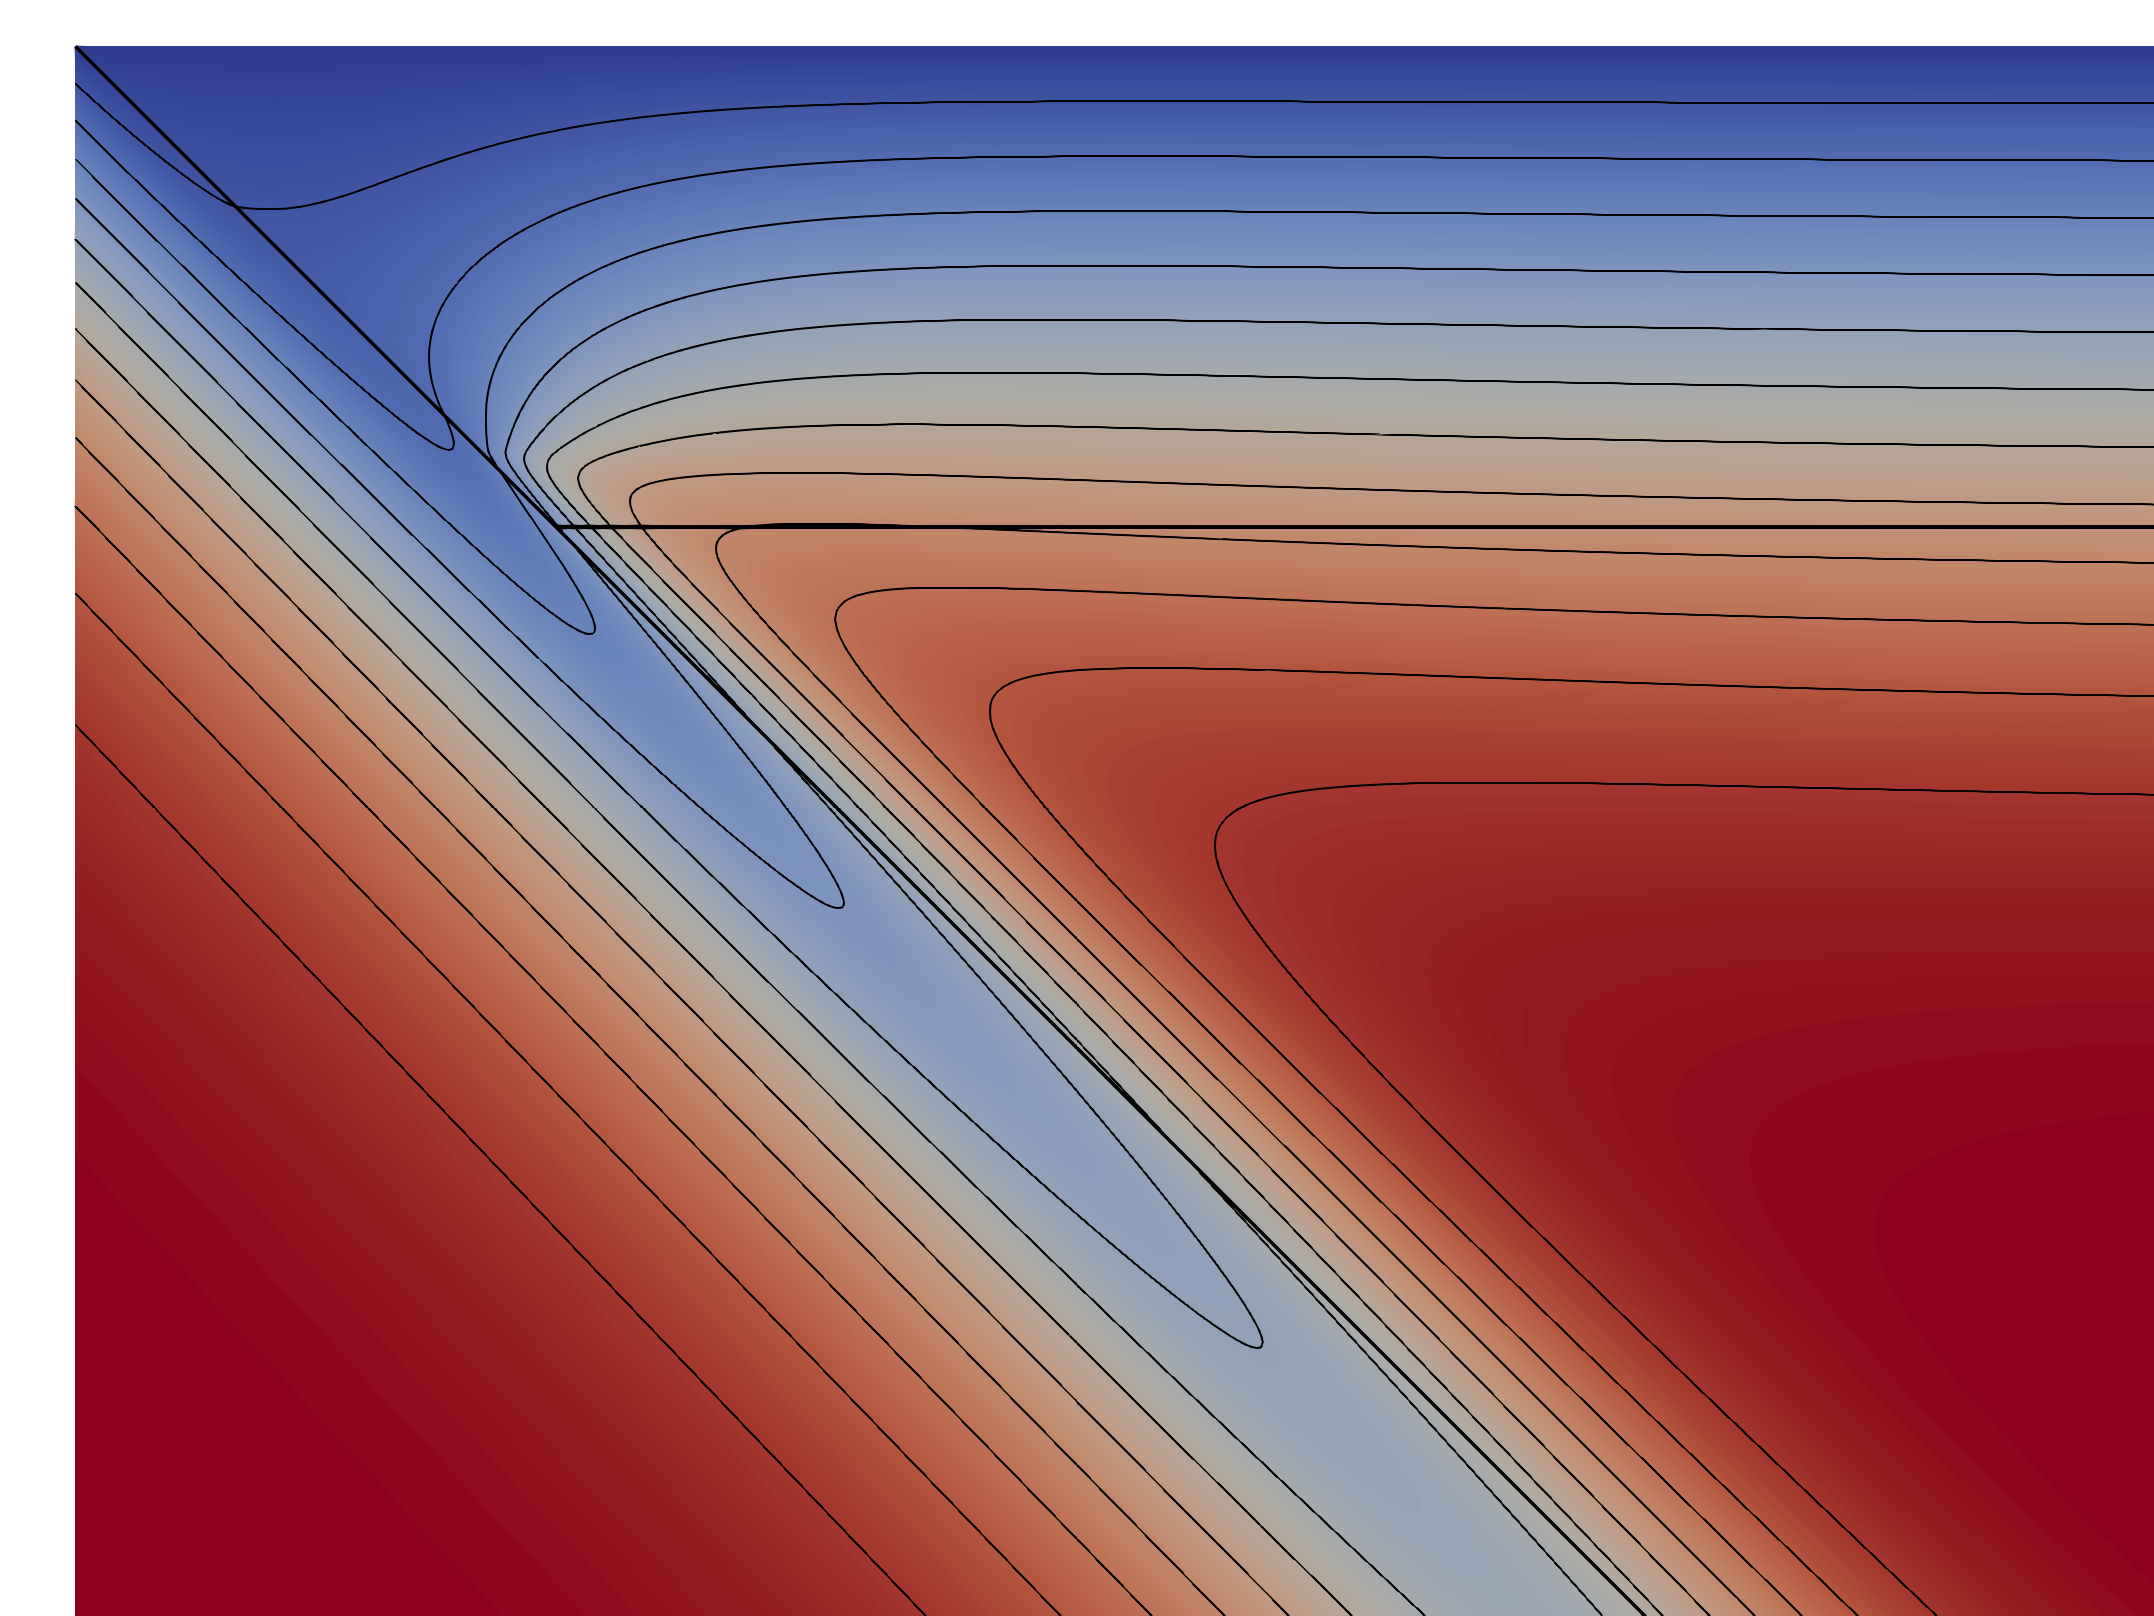
\includegraphics[width=7cm]{python_codes/fieldstone_45/images/temp_zoom}\\
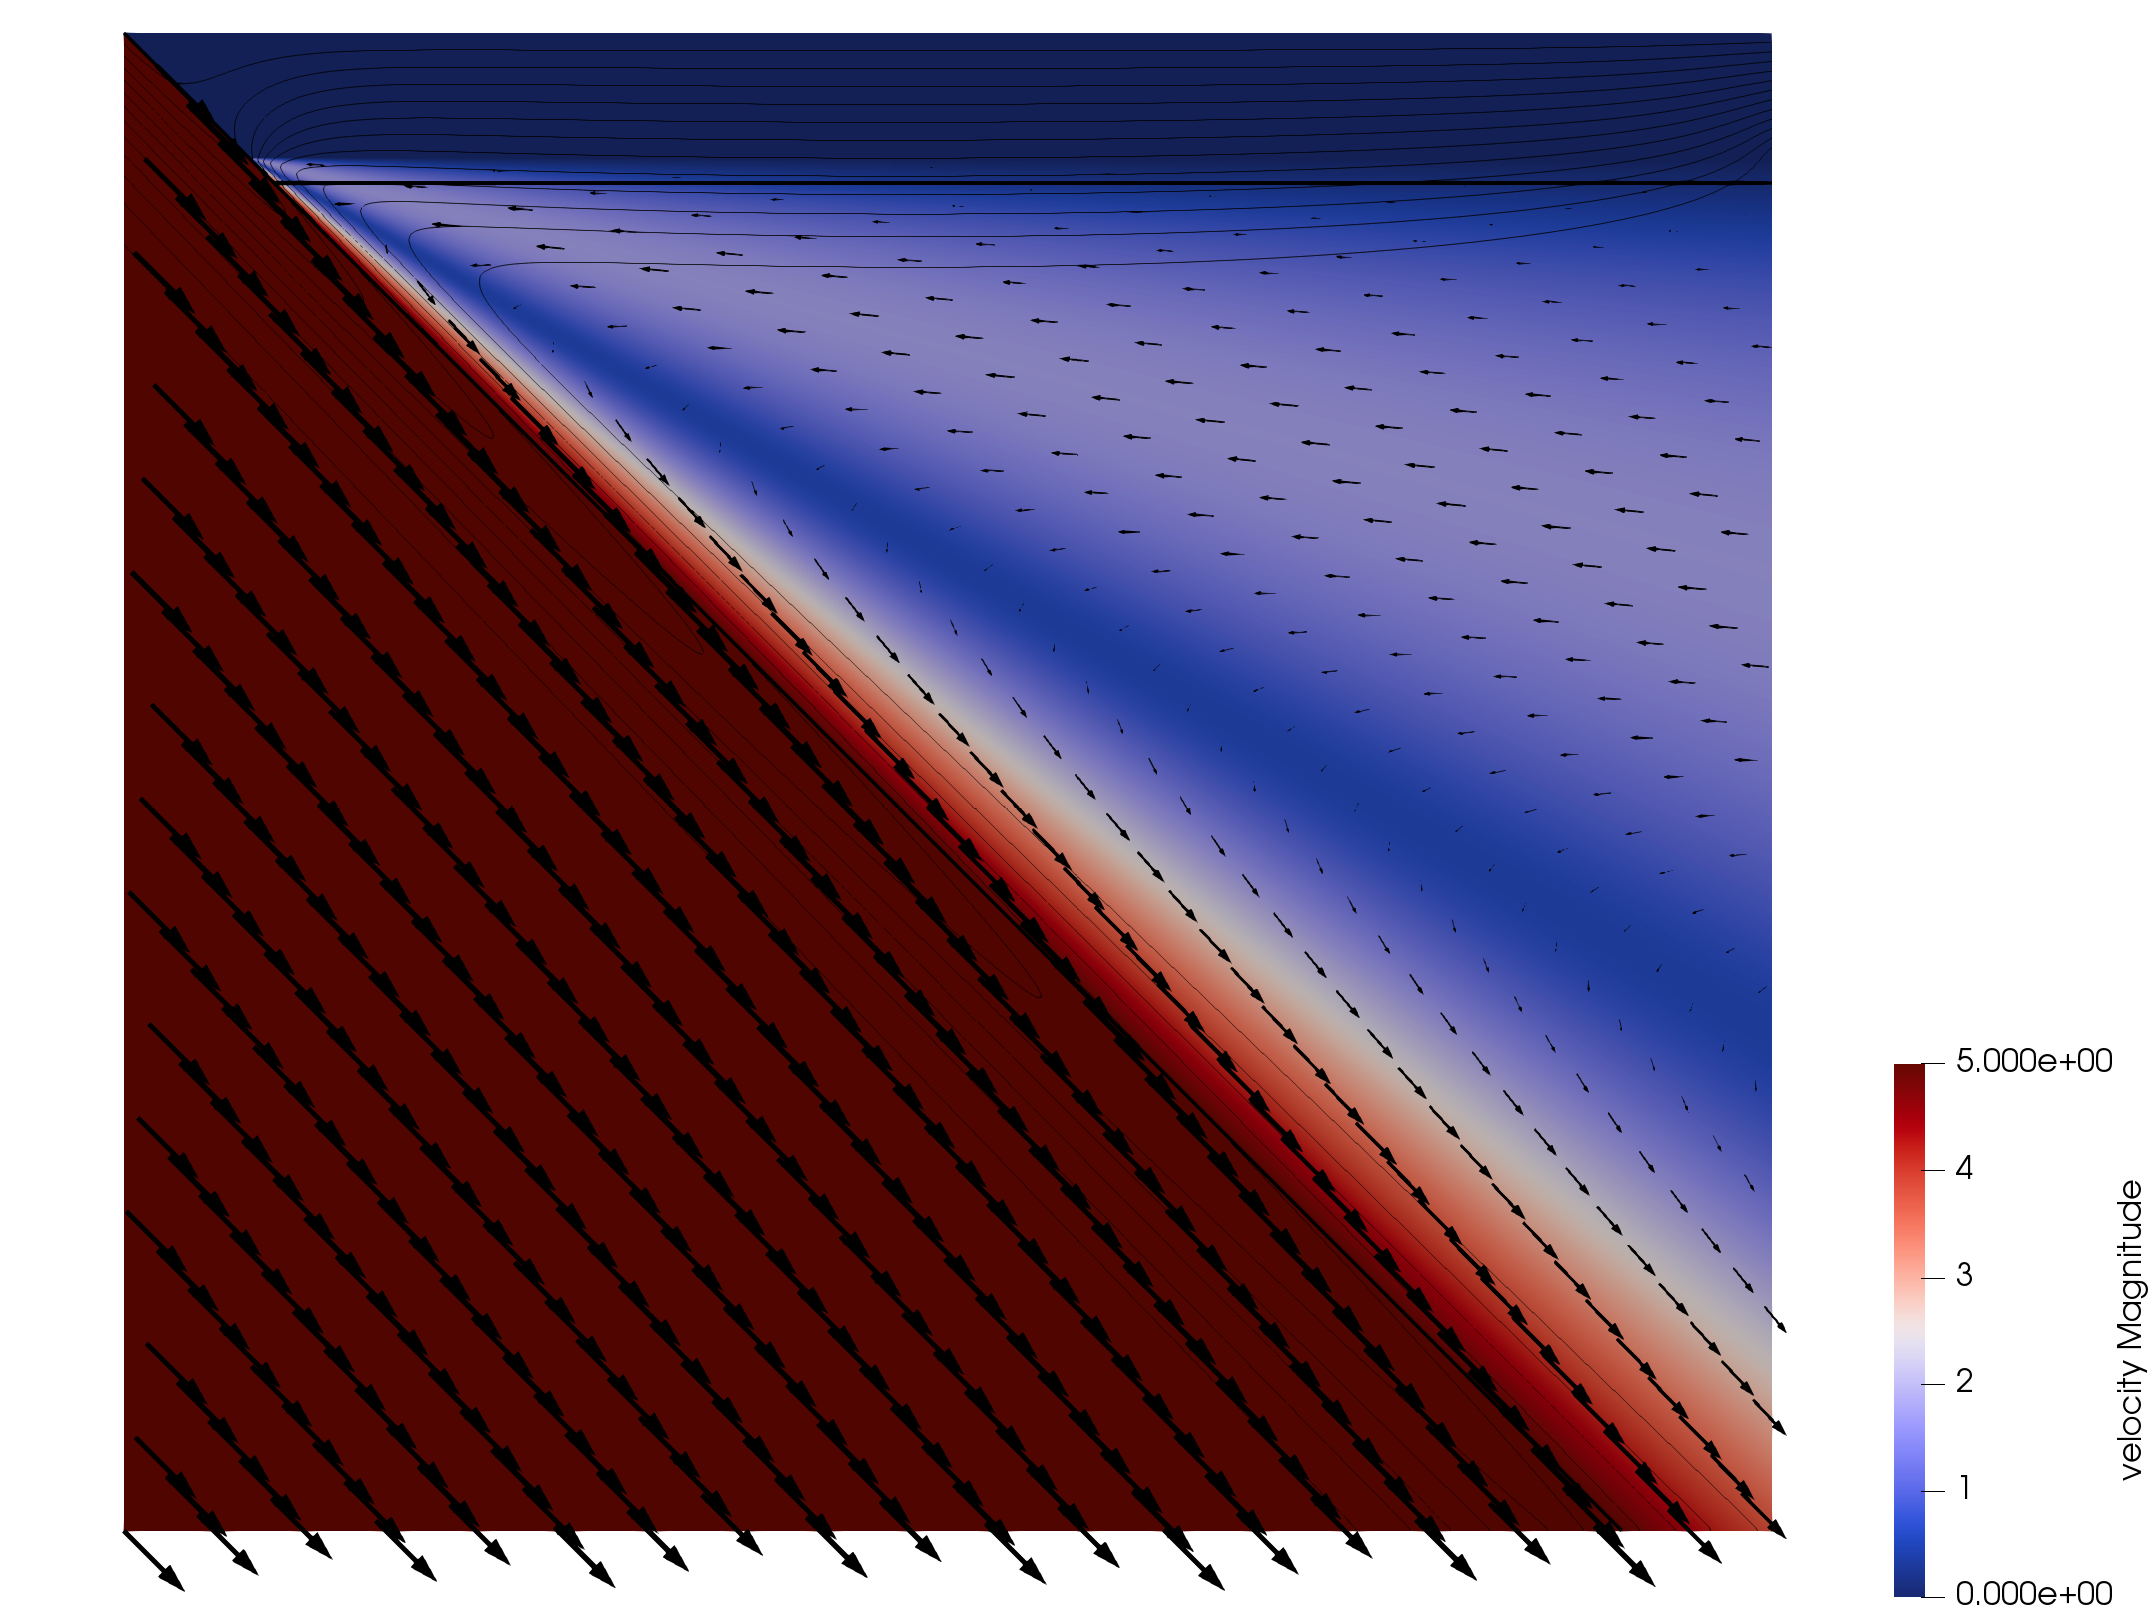
\includegraphics[width=7cm]{python_codes/fieldstone_45/images/vel}
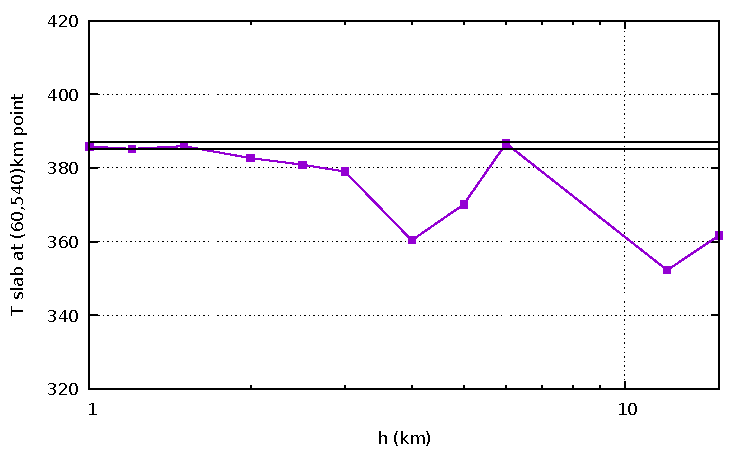
\includegraphics[width=7cm]{python_codes/fieldstone_45/images/T60.pdf}\\
{\small Results obtained on mesh 660x600(x2) elements. Black lines on lower right figure 
correspond to a visible range of values as shown in Fig.3a of \cite{vack08}.}
\end{center}

\begin{center}
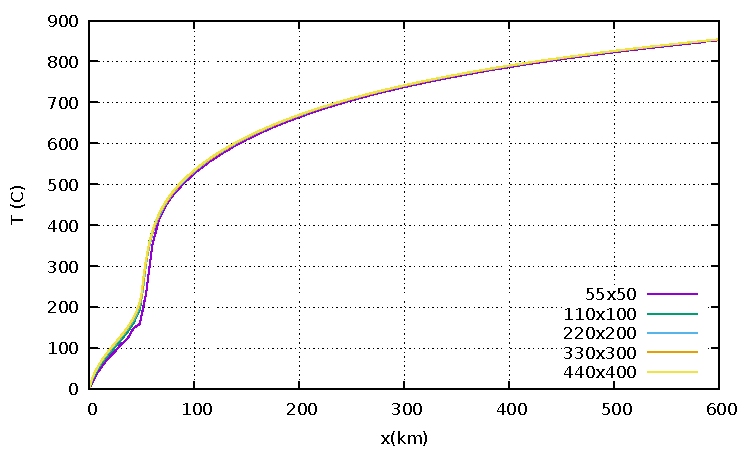
\includegraphics[width=7cm]{python_codes/fieldstone_45/images/tempdiag}
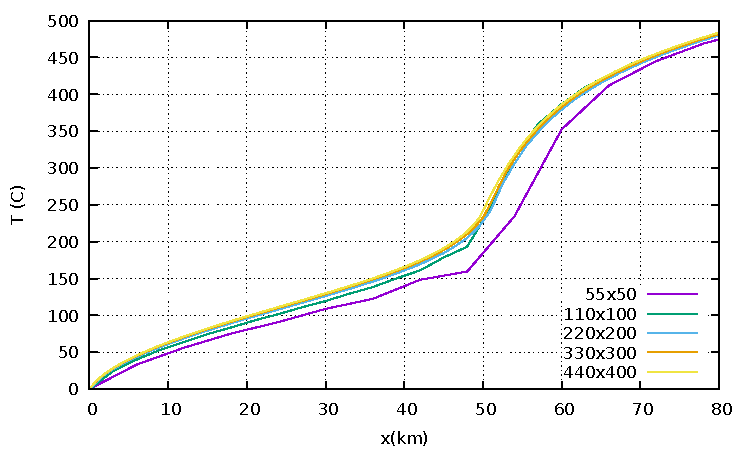
\includegraphics[width=7cm]{python_codes/fieldstone_45/images/tempdiag_zoom}\\
{\small Temperature values on the slab top surface ($y=L_y-x$) plotted as a function of the $x$ coordinate.
Left is entire slab, right is zoom on the first $70\text{km}$}
\end{center}

The average temperature 
\[
\langle T\rangle =\frac{1}{|\Omega|}\int_\Omega T \; dV
\]
is plotted in the following figure:
\begin{center}
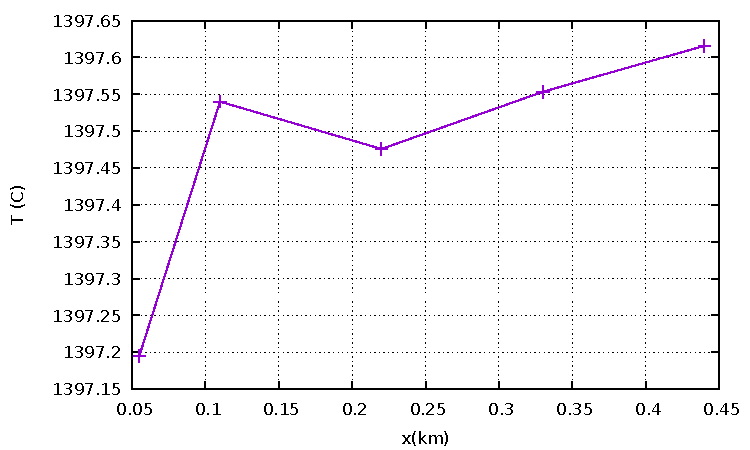
\includegraphics[width=10cm]{python_codes/fieldstone_45/images/Tavrg.pdf}\\
{\small Average temperature in the domain.}
\end{center}
We see that this measurement is not 
appropriate to assert whether the resolution is sufficient so that results converge 
to a single value, as opposed to the point wise temperature measurement presented above.
The average temperature changes by about 0.4 for an average value of about 1397, which is 
not much for a factor 12 increase in resolution (from 55x50 to 660x600).








